\documentclass[a4paper,12pt]{article}
 \usepackage{cmap}
\usepackage[utf8]{inputenc}
\usepackage[english,russian]{babel}
\usepackage[T2A]{fontenc}
\usepackage{amssymb}
\usepackage{amsmath}




\usepackage[
  a4paper, mag=1000, includefoot,
  left=1.1cm, right=1.1cm, top=1.2cm, bottom=1.2cm, headsep=0.8cm, footskip=0.8cm
]{geometry}



\usepackage{amsmath}
\usepackage{amssymb}
\usepackage{times}
\usepackage{mathptmx}
\usepackage{graphicx}

\IfFileExists{pscyr.sty}
{
  \usepackage{pscyr}
  \def\rmdefault{ftm}
  \def\sfdefault{ftx}
  \def\ttdefault{fer}
  \DeclareMathAlphabet{\mathbf}{OT1}{ftm}{bx}{it} % bx/it or bx/m
}


\mathsurround=0.1em
\clubpenalty=1000%
\widowpenalty=1000%
\brokenpenalty=2000%
\frenchspacing%
\tolerance=2500%
\hbadness=1500%
\vbadness=1500%
\doublehyphendemerits=50000%
\finalhyphendemerits=25000%
\adjdemerits=50000%
\newcommand {\pp} {\partial}
\newcommand {\ppr} [4] {\frac{\pp {#1} ^{#2}}{\pp {#3} ^{#4}}}
\newcommand {\cd} {\cdot}
\newcommand {\SL} {\implies}
\newcommand {\HD} {\hdots}
\newcommand {\FI} {\varphi}
\newcommand {\eps} {\epsilon}
\newcommand {\we} {\wedge}
\newcommand {\st} {\longleftarrow}
\newcommand {\titt} {\Longleftrightarrow}
\newcommand {\trr} {\blacktriangleright}
\newcommand {\trl} {\blacktriangleleft}
\newcommand {\iii} {\int\limits}
\newcommand {\ido} {\iint\limits} 
\newcommand {\AL} {\alpha}
\newcommand {\AS} {\alpha'}
\newcommand {\ppp}[2] {\ppr{x}{#1}{x}{#2}}
\newcommand {\LS} {\sum\limits}
\newcommand {\bb} {\mathbb}
\newcommand {\ta} {\theta}
\newcommand {\TA} {\Theta}
\newcommand {\tit} {\textit}
\newcommand {\pt} {\ppr{}{}{\ta}{}}



\begin{document}
\large
\author{- - - - - - - - - - - - - - - - ME - - - - - - - - - - - - - - - -}
\title{урчп опр форм}
\date{\today}
\maketitle


\newpage


\tableofcontents
\newpage

\section{определения}
\begin{enumerate}
\item \textit{Уравнением в частных производных} называется соотношение \\$\Phi(x_i, u, \frac{\pp u}{\pp x_i}, ..., \frac{\pp^k u}{\pp x_1^{\AL_1}...\pp x_n^{\AL_n}}) = 0$
\item Уравнение в частных производных называется квазилинейным, если $\Phi$ линейна по СТАРШИМ производным $u$
\item Уравнение в частных производных называется линейным, если $\Phi$ линейна по ВСЕМ производным $u$
\item Линейным уравнением второго порядка называется уравнение вида:
$$\LS_{i,j = 1}^n a_{i,j} u_{x_i x_j} + \LS_{i=1}^n b_i u_{x_i} +cu = f$$,где $(a_{i,j}) = A, b_i = b; a_{i,j}(x), b_i(x), c(x) \in C(Q)$
\item $u(x)\in C^2(\mathbb{R}^n)$ и удовлетворяет в обычном смысле уравнению называется решением (классическим).
\item Задача нахождения решения уравнения $\AL u = f$, удовлетворяющего условию $u|_{S_0} = u_0(x), \frac{\pp u}{\pp l}|_{S_0} = u_1(x)$ называется задачей Коши (локальной)
\item 
$$\LS_{i,j = 1}^n a_{i,j} u_{x_i x_j} + \LS_{i=1}^n b_i u_{x_i} +cu = f \quad\quad\quad(1)$$
$$u|_S=u_0, \frac{\pp u}{\pp l}|_S = u_1 \quad\quad\quad(2)$$
Пусть $S\in C^1, S = \{x: F(x) = 0\}$. Тогда $x \in S$ называется характеристической для уравнения (1), если $(A(x)\nabla F(x), \nabla F(x)) = 0$
\item Поверхность $S$ называется характеристической для (1), если каждая её точка характеристическая.

\item 

\begin{equation*}
 \begin{cases}
   \LS_{i,j = 1}^n a_{i,j} u_{x_i x_j} + \LS_{i=1}^n b_i u_{x_i} +cu = f \quad\quad\quad(1),
   \\
	(A(x)\nabla F(x), \nabla F(x)) \ne 0,
	\\
	u|_S=u_0, \frac{\pp u}{\pp l}|_S = u_1 \quad\quad\quad\quad\quad\quad\quad\quad(2)
 \end{cases}
\end{equation*}

Задача (1),(2) называется нехарактеристической задачей Коши.


\item Функция $g$ называется аналитической в точке $x_0\in Q$, если существует $U(x_0)\subset Q$, такая, что $\forall x \in U(x_0): $\\$g(x) = \LS_{\AL_1=0}^\infty ... \LS_{\AL_n=0}^\infty g_{\AL_1 ... \AL_n} (x_1 - x_{0,1})^{\AL_1} ... (x_n - x_{0,n})^{\AL_n} = \LS_{|\AL|=0}^\infty g_\AL (x-x_0)^\AL$ и ряд сходится абсолютно.

\item аналитическая в точке $x_0\in Q$ функция $\widetilde{g}(x)$ называется мажорантой функции $g(x)$, если $\forall \AL, 0 \leq |\AL|< \infty: |g_\AL| \leq \widetilde{g}_\AL$

\item 
\begin{equation*}
 \begin{cases}
   u_{y_ny_n} = \LS_{i,j=1}^n {p}_{i,j} V_{y_iy_j}+\LS_{i=1}^n{q}_iV_{y_i} + {s}u + {f} \quad\quad\quad(5),
   \\
	u|_S = {u_0},
	\\
	u_{y_n}|_S = {{u_1}}\quad\quad\quad\quad\quad\quad\quad\quad\quad\quad\quad\quad\quad\quad\quad(8)
 \end{cases}
\end{equation*}

Пусть у нас имеется задача
\begin{equation*}
 \begin{cases}
   V_{y_ny_n} = \LS_{i,j=1}^n \widetilde{p}_{i,j} V_{y_iy_j}+\LS_{i=1}^n\widetilde{q}_iV_{y_i} + \widetilde{s}u + \widetilde{f} \quad\quad\quad(7),
   \\
	V|_S = \widetilde{V}_0,
	\\
	V_{y_n}|_S = \widetilde{{V_1}}\quad\quad\quad\quad\quad\quad\quad\quad\quad\quad\quad\quad\quad\quad\quad(8)
 \end{cases}
\end{equation*}
Задача (7),(8) является мажорирующей задачей по отношению к задаче (5),(6), если $p_{i,j}, q_i, f, s, v_0, v_1$ являются мажорантами
\item ВАЖНОЕ ЗАМЕЧАНИЕ\\
решение мажорирующей задачи является мажорантой для решения исходной задачи

\item Классификация линейных дифференциальных уравнений второго порядка.\\
$\LS_{i,j = 1}^n a_{i,j} u_{x_i x_j} + \LS_{i=1}^n b_i u_{x_i} +cu = f$\\
если $a_{ij}\ne a_{ji}$, то новые $\widetilde{a}_{ij} = \widetilde{a}_{ji} = \frac{a_{ij} + a_{ji}}{2}$\\
У новой матрицы нет жордановых клеток!\\
есть $n$ с.з. $\lambda_1,...,\lambda_n$
1) Уравнение называется эллиптическим в точке $x_0$, если $n_+ = n$, или $n_- = n$\\
2) гиперболический, если $n_+ = 1, n_- = n-1$, или $n_- = 1, n_+ = n-1$\\
3) параболическим, если $n_0 > 0$\\
4) гипергиперболическим, если $n_0 = 0, n_+ \ge 2, n_- \ge 2$\\\\
($n_-, n_0, n_+$ - число отрицательных, равных 0, и положительных СЗ)\\\\ ПРИ ЗАМЕНЕ ПЕРЕМЕННЫХ ТИП УРАВНЕНИЯ СОХРАНЯЕТСЯ!!!!!\\
\item $F(x,y)$ является интегралом дифференциального уравнения $a_{11}\left(\frac{dy}{dx}\right)^2 -2a_{12}\left(\frac{dy}{dx}\right) +a_{22} = 0 \titt$ является решением уравнения $a_{11}F_x^2 + 2a_{12}F_xF_y + a_{22} = 0$\\
\item !!!! Канонический вид:\\
Гиперболический: $u_{\xi_1\xi_2} - u_{\eta_1\eta_2}= \Phi$\\
Эллиптический: $u_{\xi_1\xi_2} + u_{\eta_1\eta_2}= \Phi$\\
Параболический: $u_{\eta_1\eta_2}= \Phi$

\item Функция $u\in C^2(\mathbb{R}^n\times (0;+\infty))\cap C^1(\mathbb{R}^n\times [0;+\infty))$, удовлетворяющая волновому уравнению\\
$(1) \quad\quad \quad u_{tt} - \Delta u = f(x,t)$ и начальному условию \\$(2)\quad\quad \quad u(x,0)=\FI(x); u_t(x,0) = \psi(x)$ называется классическим решение задачи Коши для уравнения (1)


\item $lX = (pX')'+qX, p\in C^1([0,a]), 0 < p_0\le p(x), q(x) \in C([0,a]), q(x) \le 0$- дифференциальное выражение, $X = X(x)$.\\
Функция $X\not\equiv0: X\in C^2((0,a))\cap C([0,a]): $ для некоторого $\lambda: lX = \lambda X, X(0)=X(a) = 0$, называется собственной функцией к задача Щтурма-Лиувилля, а $\lambda$ - с.з.

\item Функцией Грина задачи Штурма-Лиувилля называется функция $G(x,y):$\\
1) $G(x,y)\in C([0,a]^2)$\\
2) $G(0,y) = G(a,y) = 0 \quad\quad(y\in(0,a))$\\
3) при $x\ne y G_x, G_{xx}$ непрерывны и $(p(x)G_x)_x + qG = 0\forall y\ne x$\\
4) $\forall x\in(0,a): p(x)(G_x(x+0,x)-G_x(x-0,x))=1$ 
\item уравнение теплопроводности\\
$u_t - \Delta u=0, x\in  \mathbb{R}^n, t > 0, t < T$
\item Задачей Коши для уравнения теплопроводности называется функция $u(x,t)\in C^{2,1}(\mathbb{R}^n\times (0,T])\cap C(\mathbb{R}^n\times [0,T])$, удовлетворяющая уравнению $\uparrow$ и начальному условию $u(x,0)=\FI(x)$
\item Смешанная задача для $\uparrow$ - задача нахождения $u$

\item любая функция, удовлетворяющая уравнению Лапласа ($\Delta u = 0$) называется гармонической.

\item ЗАДАЧА ДИРИХЛЕ И НЕЙМАНА\\
Пусть $Q$ ограниченное открытое множество\\
$u\in c^2(Q)\cap C(\overline{Q}), \Delta u=0$
1) Дирихле: $u|_{\pp Q} = \FI$\\
2) Неймана: $\frac{\pp u}{\pp l}=\FI$


\item Функцией Грина задачи Дирихле для уравнения Лапласа называется функция вида $G(x,y) = E_n(x-y) + g(x,y)$\\
1) $\Delta_xg(x,y)=0$\\
2) $G(x,y)|_{x\in\pp Q} = 0$\\
3) $E_n$ задано выше (а где блинб????)


\item Функция u называется слабым решением З.К. если \\
1) $u -\FI\in \stackrel{0}{H^1}(Q)$
2) $\forall v\in \stackrel{0}{H^1}(Q): \iii_Q (\nabla u, \nabla v)dx = -\iii_Q (f,v)dx$

\item Функция u называется слабым решением З.Н. если \\
1) $u -\FI\in \stackrel{0}{H^1}(Q)$
2) $\forall v\in \stackrel{0}{H^1}(Q): \iii_Q (\nabla u, \nabla v)dx = \iii_\Gamma \FI v ds-\iii_Q fvdx$







\end{enumerate}




\newpage
\section{формулировки}

\begin{enumerate}
\item Теорема Коши-Ковалевской\\
Пусть задача Коши аналитична (то есть $a_{i,j}, b_i, c, f, F, u_0, u_1$  аналитичны), $\forall x \in S (A\nabla F, \nabla F) \ne 0$. Тогда $\forall x_0\in S \exists U(x_0)$, в которой существует аналитическое решение, и ни в какой окрестности не существует другого аналитического решения.


\item Глобальная теорема Коши-Ковалевской\\
Пусть $Q$ - область, $S$ - поверхность, которая делит $Q$ на $Q_+$ и $Q_-$ Рассмотрим задачу:\\
\begin{equation*}
 \begin{cases}
   \LS_{i,j=1}^n a_{ij} u_{x_ix_j} + \LS_{i=1}^n b_i u_{x_i}+cu=f \quad\quad\quad(1)
   \\
	u|_S = u_0,
	\\
	u_{y_n}|_S = {{u_1}}\quad\quad\quad\quad\quad\quad\quad\quad\quad\quad\quad\quad\quad\quad\quad(2)
\end{cases}
\end{equation*}
$F=0; (\nabla F, l) \ne 0$\\
Пусть задача (1),(2) аналитична и $(A\nabla F,\nabla F) \ne 0$ на $S$. Тогда существует $Q'\subset Q, S\subset Q'$ и в $Q'$ задача имеет аналитическое решение и ни в какой областиЮ содержащей $S$, задача не имеет более одного аналитического решения.
\item Задача Коши для волнового уравнения имеет не более одного классического решения.
\item Пусть $\psi(x)\in C^k(\mathbb{R}^3), k = 0, 1, 2,...$, тогда $u_\psi \in C^k(\mathbb{R}^3 \times [0;+\infty))$, При $k \ge2: u_\psi$ является классическим решением задачи Коши. Кроме того, $\Delta u_\psi(x,0) = 0$
\item Формула Кирхгофа ($n=3$):
$$u = \frac{1}{4\pi t}\iii_{|x-\xi|=t}\psi(\xi)ds_\xi + \frac{\pp}{\pp t} \left(  \frac{1}{4\pi t}\iii_{|x-\xi|=t}\FI(\xi)ds_\xi \right)$$
\item Формула Пуассона ($n=2$):
$$u(x_1,x_2,t) = \frac{1}{2\pi}\iii_{|x-\xi|<t}\frac{\psi(\xi_1,\xi_2)d\xi_1d\xi_2}{\sqrt{t^2 - (\xi_1 - x_1)^2 - (\xi_2-x_2)^2}} + \frac{\pp}{\pp t} \left( \frac{1}{2\pi}\iii_{|x-\xi|<t}\frac{\FI(\xi_1,\xi_2)d\xi_1d\xi_2}{\sqrt{t^2 - (\xi_1 - x_1)^2 - (\xi_2-x_2)^2}} \right)$$
\item Формула Даламбера ($n=1$):
$$u(x,t) = \frac{1}{2}(\FI(x+t) + \FI(x-t)) + \frac{1}{2}\iii_{x-t}^{x+t}\psi(\xi)d\xi$$
\item С.З. к задаче Штурма-Лиувилля отрицательные вещественные.
\item $\uparrow$ Каждое подпространство, соответствующее собственному значению $\lambda$ одномерно.
\item $\uparrow$ собственные функции, отвечающие различным С.З. взаимно ортогональны в $L_2([0,a])$

\item Функция Грина существует. /*в доказательстве случайно получили что $G$ симметрична*/
\item Решение: $u(x) = \iii_0^a G(x,y)f(y)dy$
\item $T u = \iii_0^aG(x,y)u(y)dy$ - компактный самосопряженный оператор
\item Пусть $T$ - компактный самосопряженный оператор в сепарабельном Гильбертовом пространстве $H$. Тогда спектр оператора состоит из С.З, образующих последовательность с пределом в точке 0и соответствующая система функций полна и ортогональна в $H$ /*честное слово, лучше в функане*/
\item Неравенство Бесселя\\
Пусть $f = \LS_{k=1}^\infty f_kX_k, X_k$ - ортонормированная система, тогда $\LS_{k=1}^\infty c_k^2 \le \|f\|^2=\iii_0^af^2(x)dx$
\item Рассмотрим задачу\\
$p\in C^1([0,a]), 0<p_0\le p; q\in C^1([0,a]), q\le0$
\begin{equation*}
 \begin{cases}
   u_{tt} - (pu_x)_x-qu=0
   \\
	u(0,t) = u(a,t) = 0
	\\
	u(x,0)=\FI
\\
u_t(x,0)=\psi
\end{cases}
\end{equation*}
Пусть $\FI \in C^3([0,a]), \FI(0)=\FI(a)=0, L\FI(0)=L\FI(a)=0, \psi(x)\in C^2([0,a]),\psi(0)=\psi(a)=0$. Тогда смешанная задача имеет классическое решение.
\item Принцип максимума в одномерном случае.\\
$\sup\limits_{\overline{\Omega}}u(x,t) = \sup\limits_{Q, \Sigma_1, \Sigma_2}$

\begin{figure}[h!]
\center{ 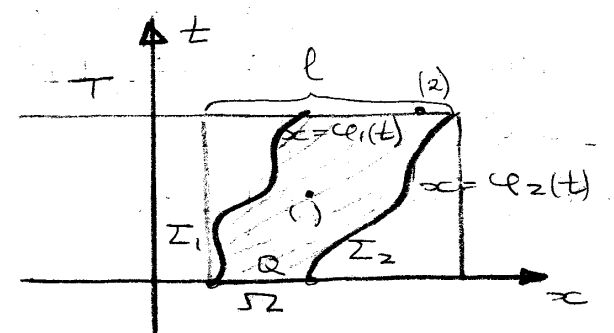
\includegraphics[width=1\linewidth]{p.png}}
\label{fig:mpr}
\end{figure}

\item Первая смешанная задача для уравнения теплопроводности не может иметь более одного классического решения в ограниченной области /// бонус: доказательство. вычли из одного другое и получили 0 на границе и дальше принцип максимума значит совпали.
\item Теорема о скорости убывания решений.\\
Пусть $h(x,t)=0$ и $Q$ ограничена. Тогда $\sup\limits_Q|u(x,t)|\to 0, t\to\infty$
\item Теорема формула Пуассона\\
Пусть $\FI\in C(\mathbb{R}^n)$ и $\exists M>0: |\FI(x)| \le M, x\in \mathbb{R}^n$, тогда
$$u(x,t) = \left(\frac{1}{2\sqrt{\pi t}}\right)^n \cdot \iii_{\mathbb{R}^n}exp\left(-\frac{|x-\xi|}{4t}\right) \FI(\xi)d\xi$$
определяет классическое решение задачи.
\item стабилизация решений задачи Коши для уравнения теплопроводности.\\
Пусть $\lim\limits_{x\to+\infty} \FI(x)= \FI_+, \lim\limits_{x\to-\infty} \FI(x)= \FI_-$, тогда $\lim\limits_{t\to+\infty} \FI(x,t)= \frac{\FI_+ + \FI_-}{2}$
\item Лемма Римана-Лебега\\
Пусть $I\subset \mathbb{R}$ - интервал, $f\in L_1(I)$, тогда $\iii_If(x)\cos(\lambda x)dx\to0, \iii_If(x)\sin(\lambda x)dx\to0$ при $\lambda\to\infty$


\item принцип максимума/*шо опять???*/\\
Пусть $Q$ - ограниченная область, $u\in C^2(Q)\cap (\overline{Q}), \Delta u=0$. Тогда $\max\limits_{\overline{Q}}u=\max\limits_{\pp Q}u$
\item усиленный принцип максимума/*если ты ещё тут, то не позорься, открой комплан*/\\
Пусть $Q$ - ограниченная область, $u\in C^2(Q)\cap (\overline{Q}), \Delta u=0$. Если существует точка внутри, где достигается максимум по границе, то это константа.


\item Классическое решение задачи Дирихле в ограниченной области единственно ($\le 1$)
\item Решение задачи Дирихле непрерывно зависит  от граничной функции.

\item $0=\iii_{\pp Q} \FI ds$ - необходимое условие существование решения задачи Неймана.

\item Пусть $Q$ -ограниченная область, удовлетворяющая внутреннему условию шара, тогда любые два решения задачи Неймана отличаются на постоянную.

\item Функция Грина единственна (в ограниченной)
\item Функция Грина симметрична ($G(x,y) = G(y,x)$)
\item $u(x_0) = \iii_{\pp Q} u(x) \frac{\pp G(x,x_0)}{\pp v_x}ds_x$
\item $u(x_0) = \frac{1}{2\pi R}\iii_\Gamma\FI(x) \frac{R^2-|x_0|^2}{|x-x_0|^2}ds_x$-формула Пуассона для $n=2$
\item Теорема о среднем\\
Пусть $n\ge 2, u\in C^2(B_R(0))\cap C(\overline{B_R(0)}), \Delta u=0$, тогда $$u(0)=\frac{1}{w_{n-1}R^{n-1}}\iii_{S_R(0)}u(x)ds_x$$
\item Теорема о среднем$^2$\\
Пусть $n\ge 2, u\in C^2(B_R(0))\cap C(\overline{B_R(0)}), \Delta u=0$, тогда $$u(0)=\frac{1}{|B_R(0)|}\iii_{B_R(0)}u(x)dx$$
\item неравенство Харнака\\
Пусть $u(x)\in C^2(B_R(0))\cap C(\overline{B_R(0)}), \Delta u =0, u\ge 0$, тогда для любого $x$:
$$\frac{R^{n-2}(R^2-r^2)}{(R+r)^n}u(0) \le u(x)\le\frac{R^{n-2}(R^2-r^2)}{(R-r)^n}u(0)$$
\item Теорема об устранимой особенности
Пусть $\{0\}\in Q\subset \mathbb{R}^n, n\ge2, u\in C^2(Q\setminus\{0\}), \Delta u = 0, \exists R>0, M>0: |u(x)| \le M$ в $B_R(0)$\\
Тогда функция $\widetilde{u}(x) = u(x), x \in Q\setminus 0; u_0, x=0$ из $C^2(Q); \Delta u = 0$
\item Пусть 0 в области $Q$\\
$E_2(x) = \frac{1}{2\pi}\ln|x|$\\
$E_n(x) = -\frac{r^{2-n}}{w_{n-1}}$\\
тогда существует $u_0: --||--$ непрерывная 2 и гармоническая
\item Теорема Лиувилля\\
Пусть $u:$ гармоническая и нпрерывная2 в Rn и $u(x) \ge M$\\
Тогда $u=const$
\item гармоническая и непрерывная $\in C^\infty$
\item Теорема Бернштейна...\\
Пусть $Q\subset \mathbb{R}^n$ - ограниченная область, $u$ непрерывная2 и гармоническая, $|u(x)|\le M$, тогда для любого альфа\\
$|D^\alpha u| \le M \cdot \left(\frac{n}{\delta}\right)^k \cdot k^k, k = |\AL|, \delta = dist(x,\pp Q)$

\item Пусть $u$ непрерывна2 и гармоническая. тогда она аналитична в Q
\item Теорема 1Харнака\\
Пусть $Q\subset \mathbb{R}^n, 0\in Q, u_m(x)\in C^2, \Delta u_m=0$, существует предел $u_m(0) = u_0$. тогда для любого компакта ряд равномерно сходится к $u(x)$
\item Теорема 2Харнака\\
Пусть Q- область, тогда последовательность непрерывных2 и гармонических равномерно сходится только к такой же.\\
\item Пространство Соболева полно.
\item неравенство Фридрикса.\\
Пусть Q ограниченная область, тогда существует c>0:$$\forall u\in \stackrel{0}{H^1}: \|u\|\le c\|\nabla u\|$$
\item Слабое решение задачи Коши единственно.
\item Слабое решение З.К. существует.

\item Теорема Пуассона.\\
Пусть $\FI(x)\in C(\mathbb{R}^n), |\FI(x)|\le M$, тогда классическое решение З.К.задается формулой $$u(x,t) = \left(\frac{1}{2\sqrt{\pi t}}\right)^n\iii_{\mathbb{R}^n} exp \left(-\frac{|x-\xi|^2}{ut}\right)\FI(\xi)d\xi$$

\item принцип максимума в неограниченной области для З.К.\\
$(1) u_t - \Delta u=0$\\
$(2) u(x,0) = \FI(x)$\\
Пусть $u$ - решение и $\exists N>0: |u(x,t)|\le N$\\
Тогда $\forall x\in \mathbb{R}^n, t\in [0,T]: \inf \FI(x) \le u(x,t)\le \sup \FI(x)$
\item лемма ... хз кого\\
Пусть $f\in D'(Q) \Delta f=0 /*(f,\Delta \FI)=0*/  \SL f\in C^\infty, \Delta f = 0$ в классическом смысле.







\end{enumerate}

\newpage
\section{просто полезное (нет)}
\begin{enumerate}

\item Пример Адамара оботсутствии непрерывной зависимости от начальных условий\\
$Q = \{x_1^2 + x_2^2 < 1\}$\\
Уравнение Лапласа: $u_{x_1x_1} + u_{x_2x_2} = 0$\\
$S = \{x_2 = 0\}$
$u(x_1,0) = e^{-\sqrt{n}} \cdot e^{inx_1}, u_{x_2}(x_1,0) = 0$\\
$u_{x_1x_1} = -n^2 e^{-\sqrt{n}}ch(nx_2) e^{inx_1}$\\
$u_{x_2x_2} = n^2 e^{-\sqrt{n}}ch(nx_2) e^{inx_1}$
$n\to \infty$ тогда $\frac{\pp^k}{\pp x_1^k}\to 0$\\
но если $x_2 > 0$, то не к 0, а к $\infty$


\end{enumerate}







































\end{document}

